\documentclass[en]{university}

\faculty{Department of Computer Engineering}
\course{Computer Networks}
\subject{Homework 2}
\professor{Dr. Jafari}
\student{Parsa Mohammadian}

\begin{document}

\setupdocument

\section{}
\subsection{}
\subsubsection{}
As we can see in the figure \ref{fig:WSProtocolStat}, UDP and TCP are used to transfer data over IPv4. Despite not all of the packets are used for loading \url{ce.sharif.edu}, browser had used both of them to transfer data. It used UDP for DNS queries and TCP for HTTP requests.

\begin{figure}
    \centering
    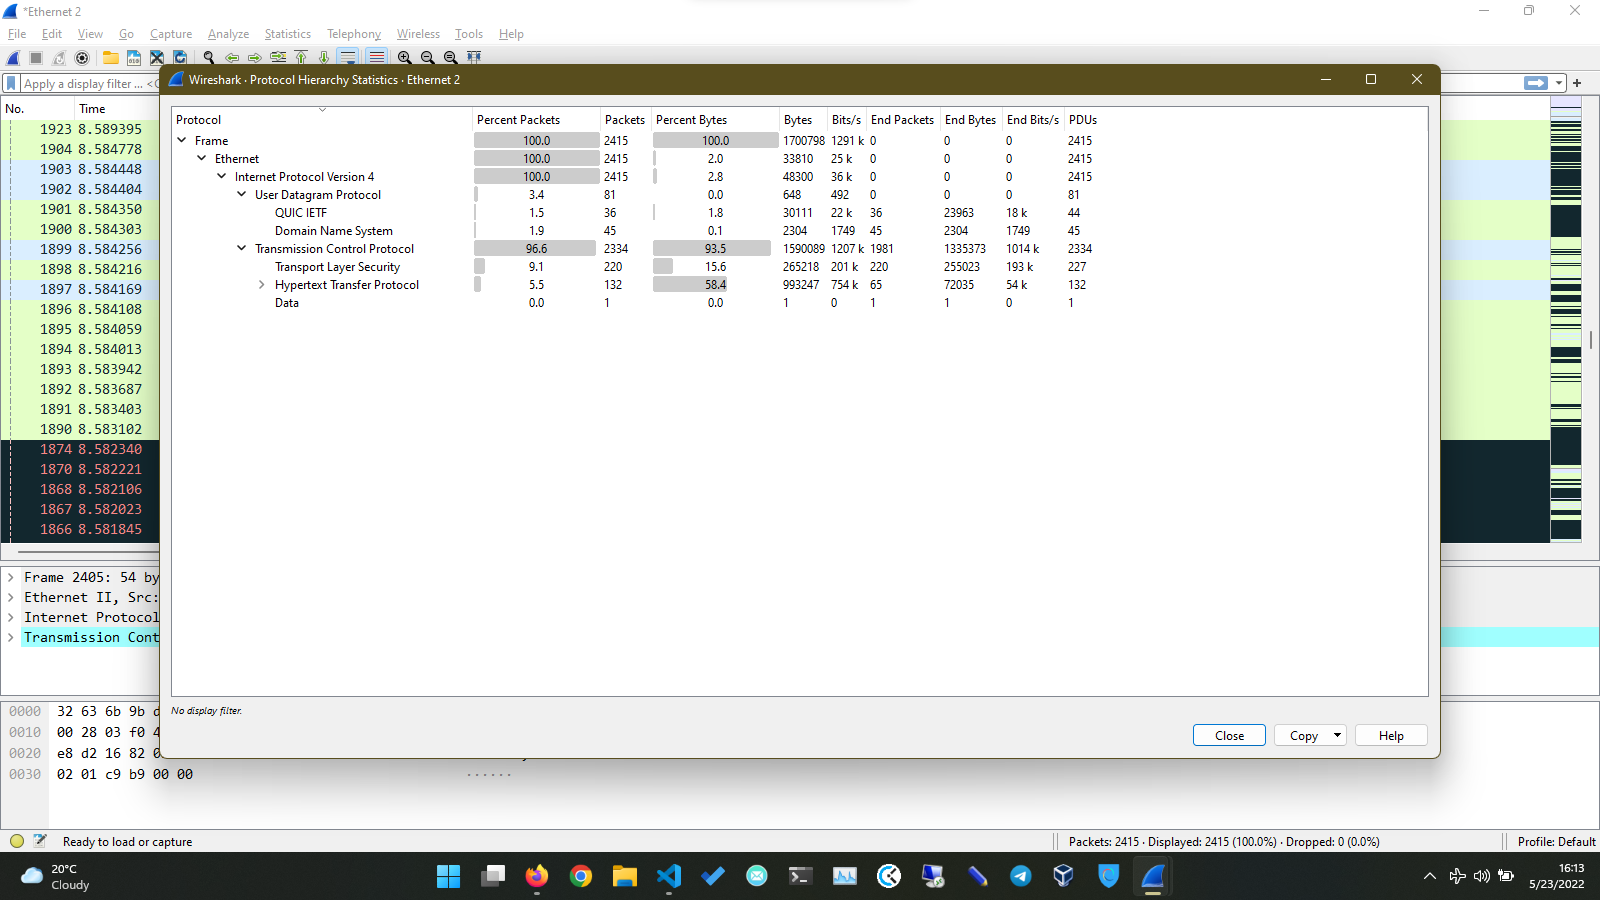
\includegraphics[width=\textwidth]{./resources/WSProtocolStat.png}
    \caption{Wireshark Protocol Statistics}
    \label{fig:WSProtocolStat}
\end{figure}

\subsubsection{}
First, we can sort the packets by the protocol type. Now we can see all of the DNS requests togehter. We can see the first DNS request for \url{ce.sharif.edu} in the figure \ref{fig:WSDNS}. As we can see, the first request is sent from \url{172.20.10.3} to \url{192.168.250.250} for A record of \url{ce.sharif.edu}. Both of these IP addresses are private LAN addresses so this request is probably to a local DNS. After that we have the second packet sent from \url{172.20.10.3} to \url{8.8.8.8} which is the Google DNS server. Then Google DNS server responds and sends the \url{81.31.168.124} as the IP address of \url{ce.sharif.edu}. After that we have exact same packets sent and received but for AAAA record; and the final response is not IP address but it is SOA record (\url{ns1.sharif.ir}) which is a record that tells the server where to find other records. After that we can see some other DNS request, like those for \url{ce.sharif.edu}, for subdomains of \url{ce.sharif.edu} which are hardware, ai, it, and web. 

\begin{figure}
    \centering
    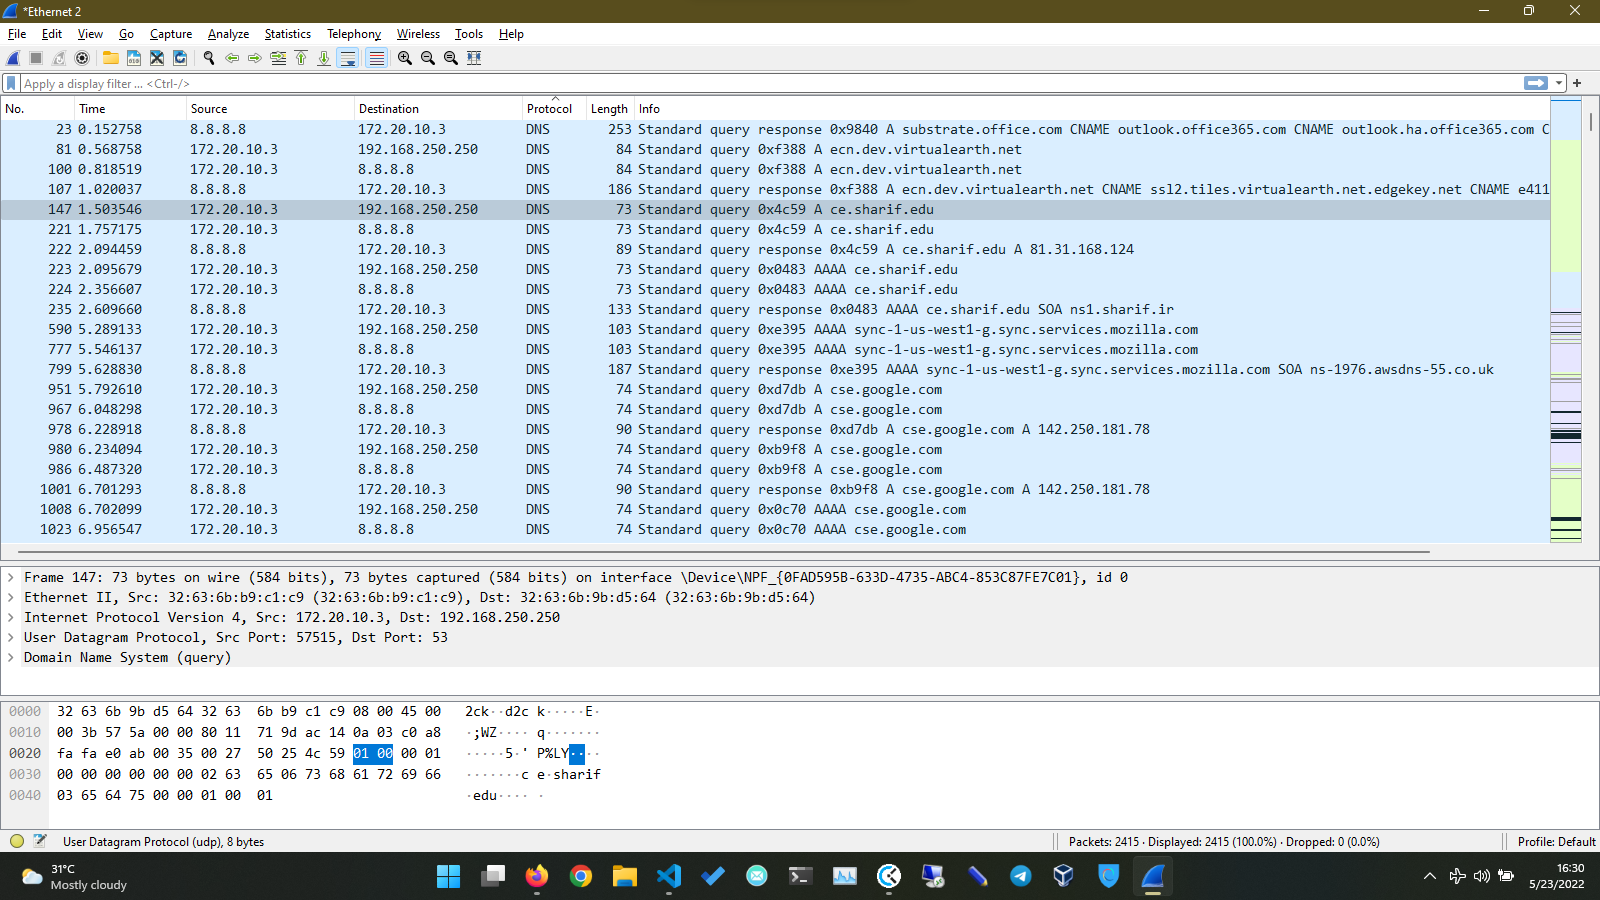
\includegraphics[width=\textwidth]{./resources/WSDNS.png}
    \caption{DNS Requests}
    \label{fig:WSDNS}
\end{figure}

\subsection{}
\subsubsection{}
As we can see in the figure \ref{fig:WSST}, there are two IP involved in the speed test process. \url{192.168.100.4} which is my local IP, and \url{81.91.144.77} which is the server for my internet connection speed test. By looking up the IP address in whois database\footnote{\url{https://who.is/whois-ip/ip-address/81.91.144.77}} we can see that the server is belonging to RIPE NCC.

\begin{figure}
    \centering
    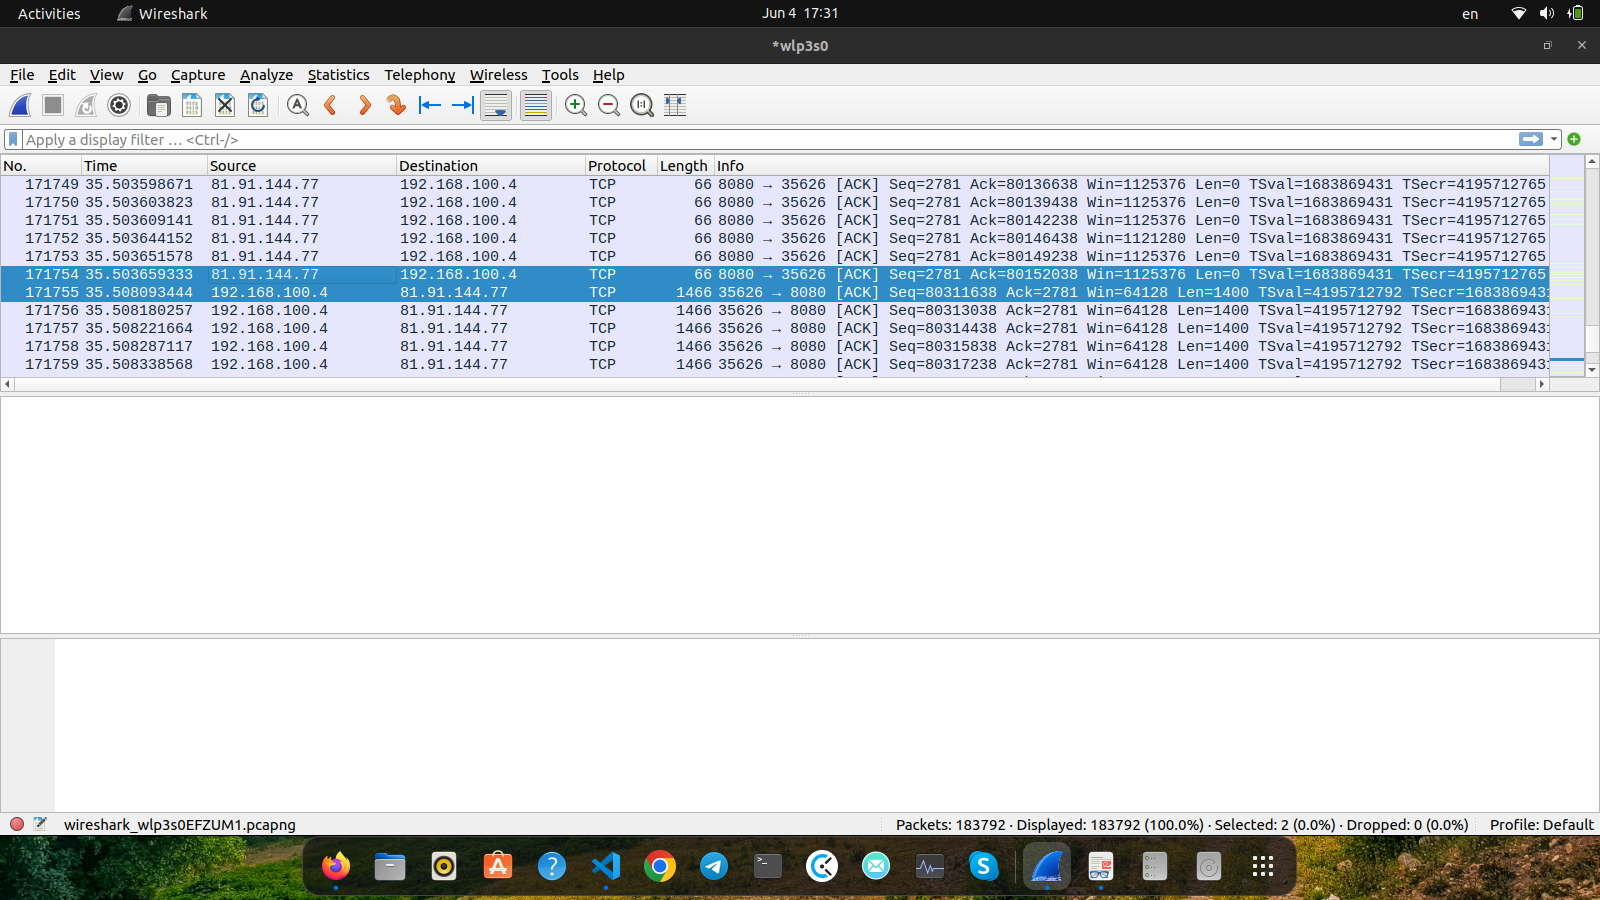
\includegraphics[width=\textwidth]{./resources/WSST.png}
    \caption{Speed Test Packets}
    \label{fig:WSST}
\end{figure}

\subsubsection{}
About 99.8\% of the packets are TCP packets. The remaining 0.2\% are UDP packets which are not used for speed test(See figure \ref{fig:WSSTP}). The reason behind using TCP for speed test is because it is reliable. Hence it take soundness of the transitioned packets into consideration. This is more ressembling to the real world situation for a normal user.

\begin{figure}
    \centering
    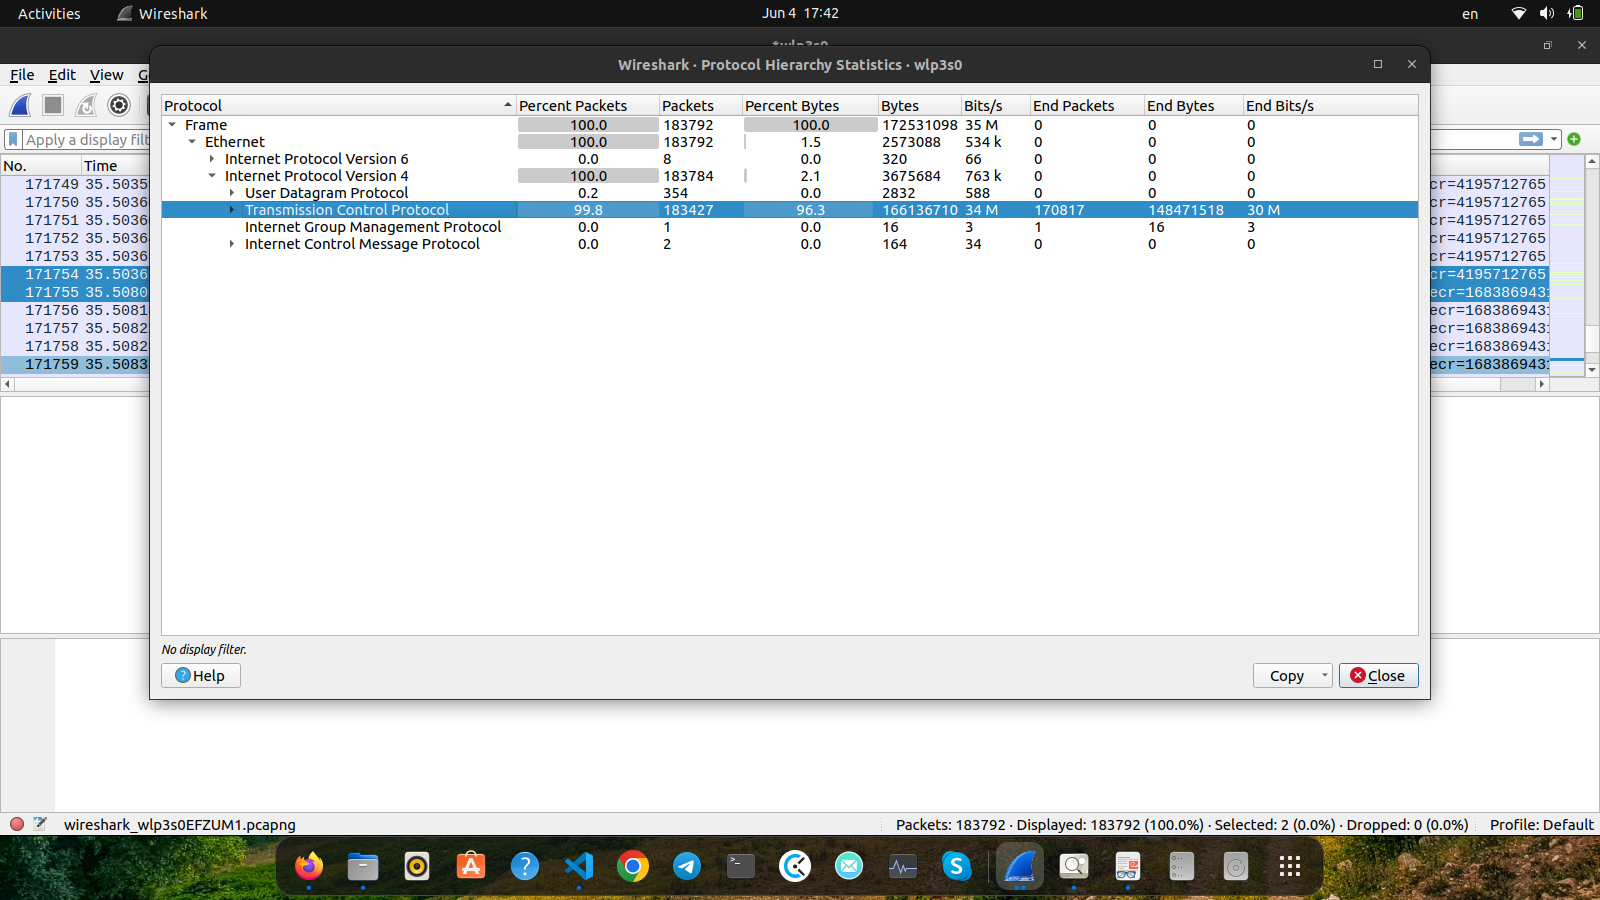
\includegraphics[width=\textwidth]{./resources/WSSTP.png}
    \caption{Speed Test Packets Protocol}
    \label{fig:WSSTP}
\end{figure}

\subsubsection{}
Delay is the amount of time that elapsed to transfer a given data. 

Bandwidth is the amount of data that is able to be transferred in a given time. In other words, it indicates the maximum capacity of the network.

Throughput is the amount of transferred data in a given time. In other words, it indicates the amount of data that is transferred successfully in a given time.

If we consider internet connection as a water pipe, then the delay is the time it takes for the water to flow from one end to the other. The bandwidth is the diameter of the pipe times length of the pipe. The throughput is the amount of water that flows through the pipe. See the figure \ref{fig:dbt}.

\begin{figure}
    \centering
    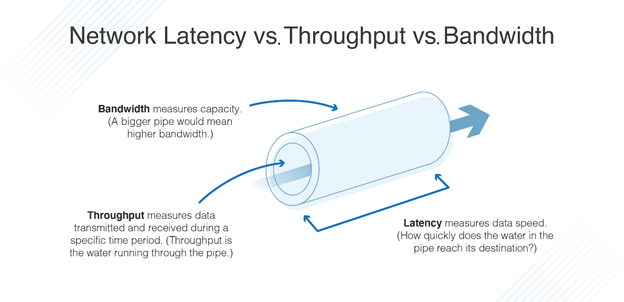
\includegraphics[width=\textwidth]{./resources/dbt.png}
    \caption{Delay, Bandwidth, and Throughput in a Water Pipe}
    \label{fig:dbt}
\end{figure}

\subsubsection{}
Using Wireshark statistics tool(\ref{fig:WSBandwidth}), we can see that the bandwidth is about 6 MB/s for both download and upload\footnote{Upload and download bandwidth are about the same in FTTH internet}, which is compilant to the speed test result.

\begin{figure}
    \centering
    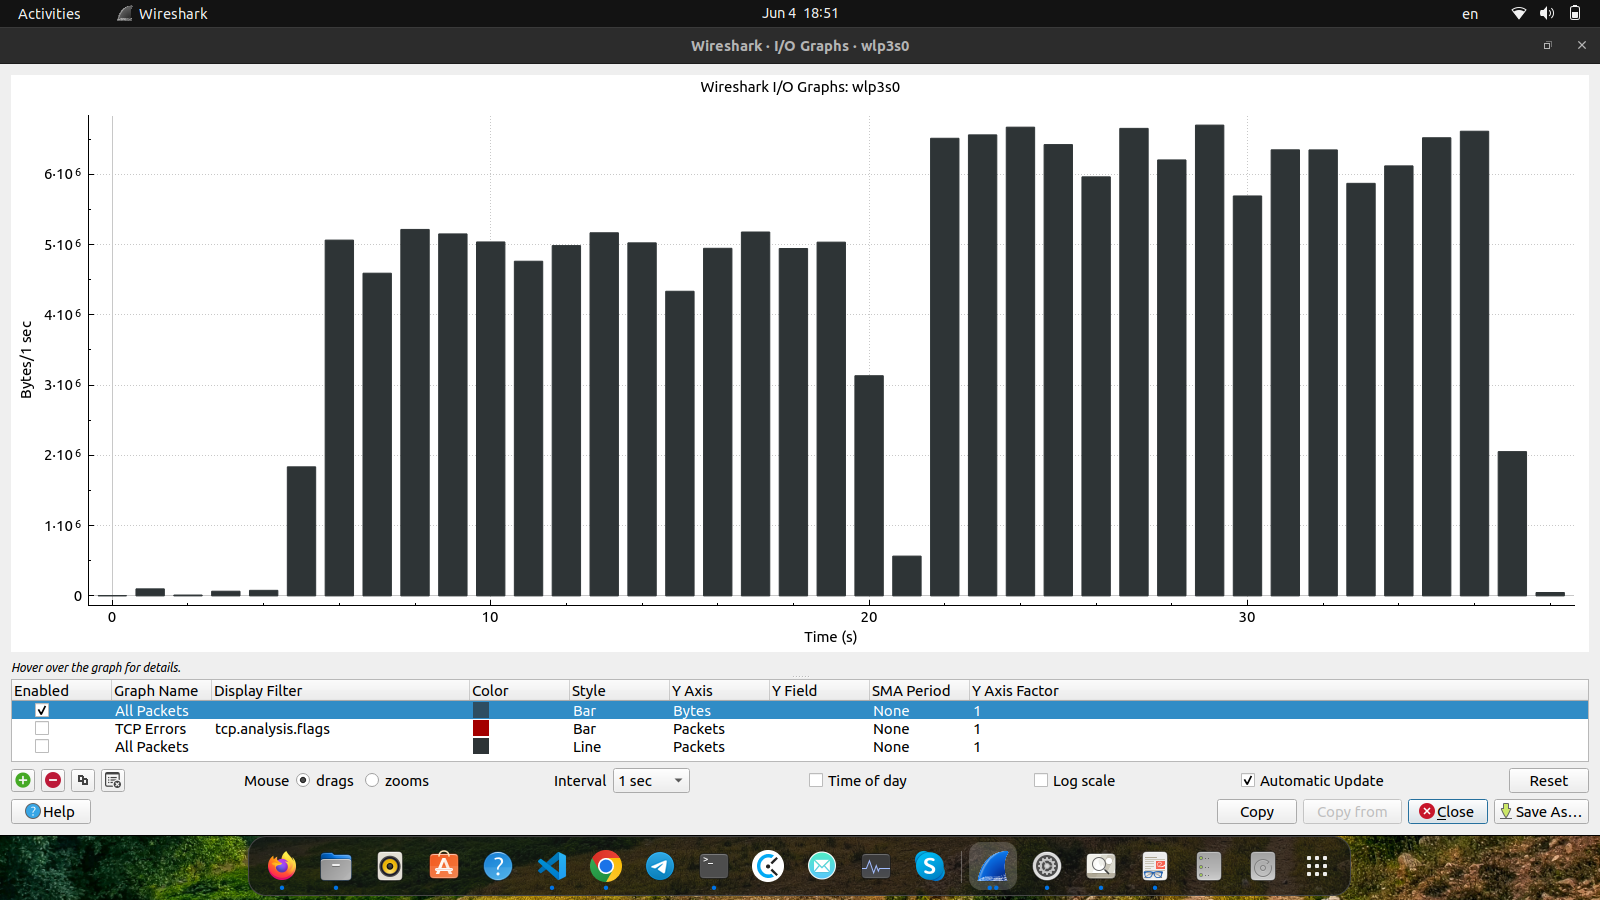
\includegraphics[width=\textwidth]{./resources/WSBandwidth.png}
    \caption{Bandwidth in Wireshark}
    \label{fig:WSBandwidth}
\end{figure}

In Wireshark by going to protocol preferences, we can turn "Calculate Conversation Timestamps" on. This appends the timestamp to the end of each packet. By opening a packet and right clicking on "Time since previous frame in this TCP stream" and chosing "Apply as Column" we can see the delay for each packet as shown in the figure \ref{fig:WSDelayEach}.

\begin{figure}
    \centering
    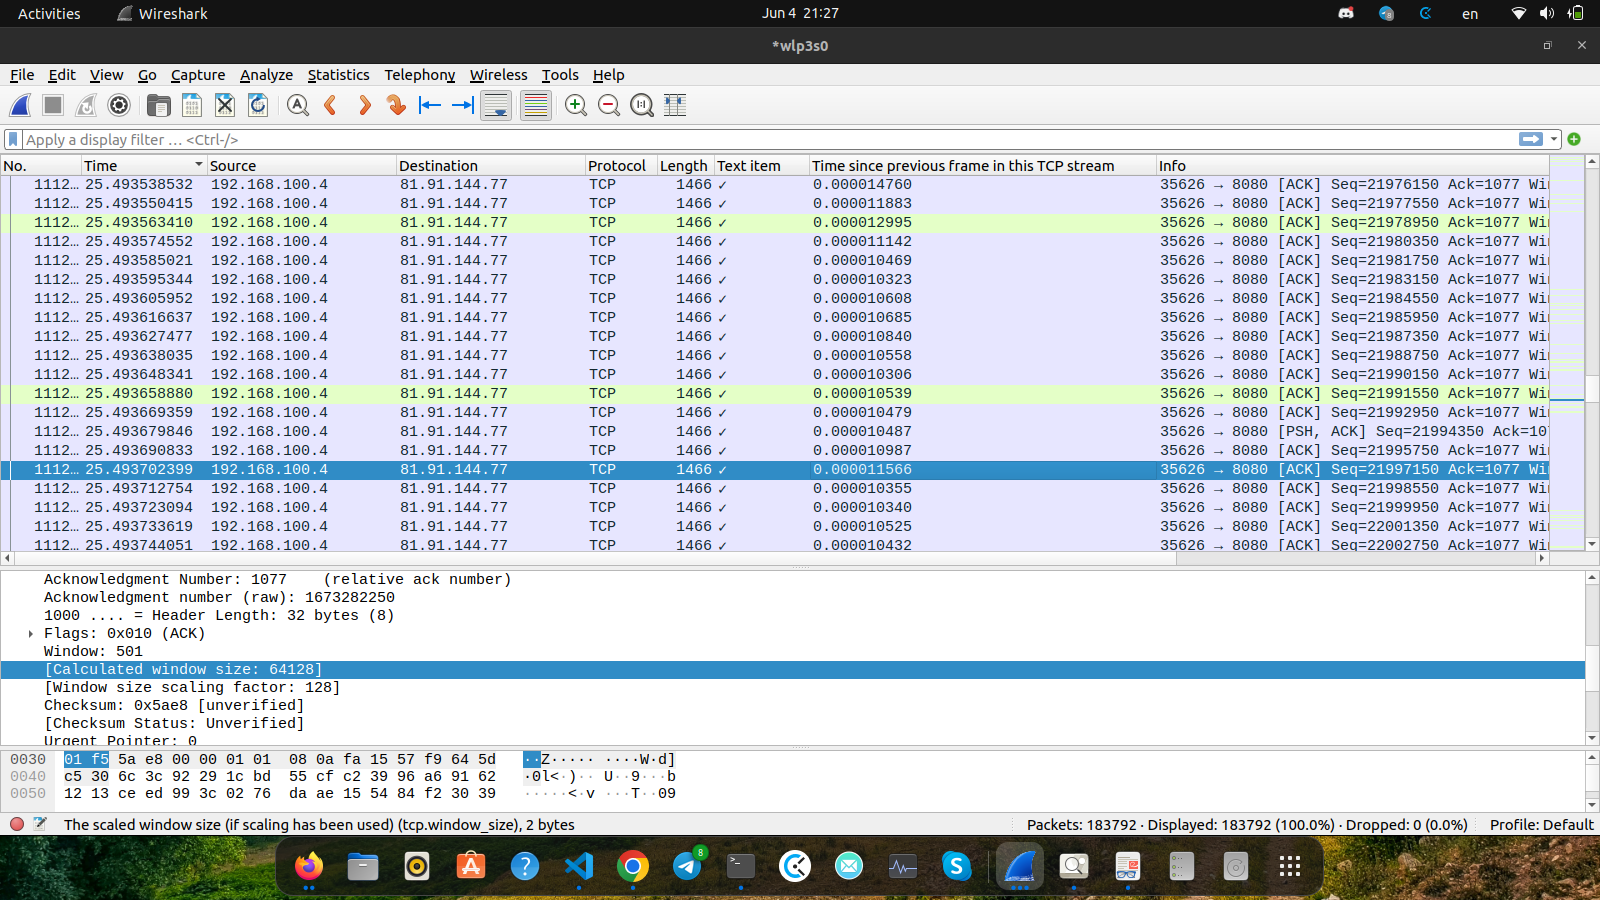
\includegraphics[width=\textwidth]{./resources/WSDelayEach.png}
    \caption{Delay for Each Packet}
    \label{fig:WSDelayEach}
\end{figure}

From statistics menu, then conversation, we can see the total time for speed test(See figure \ref{fig:WSDelayTotal}). Using these information we can calculate the throughput.

$$
    \frac{172 + 73}{33.8629} = 7.235056654923234 MB/s
$$

\begin{figure}
    \centering
    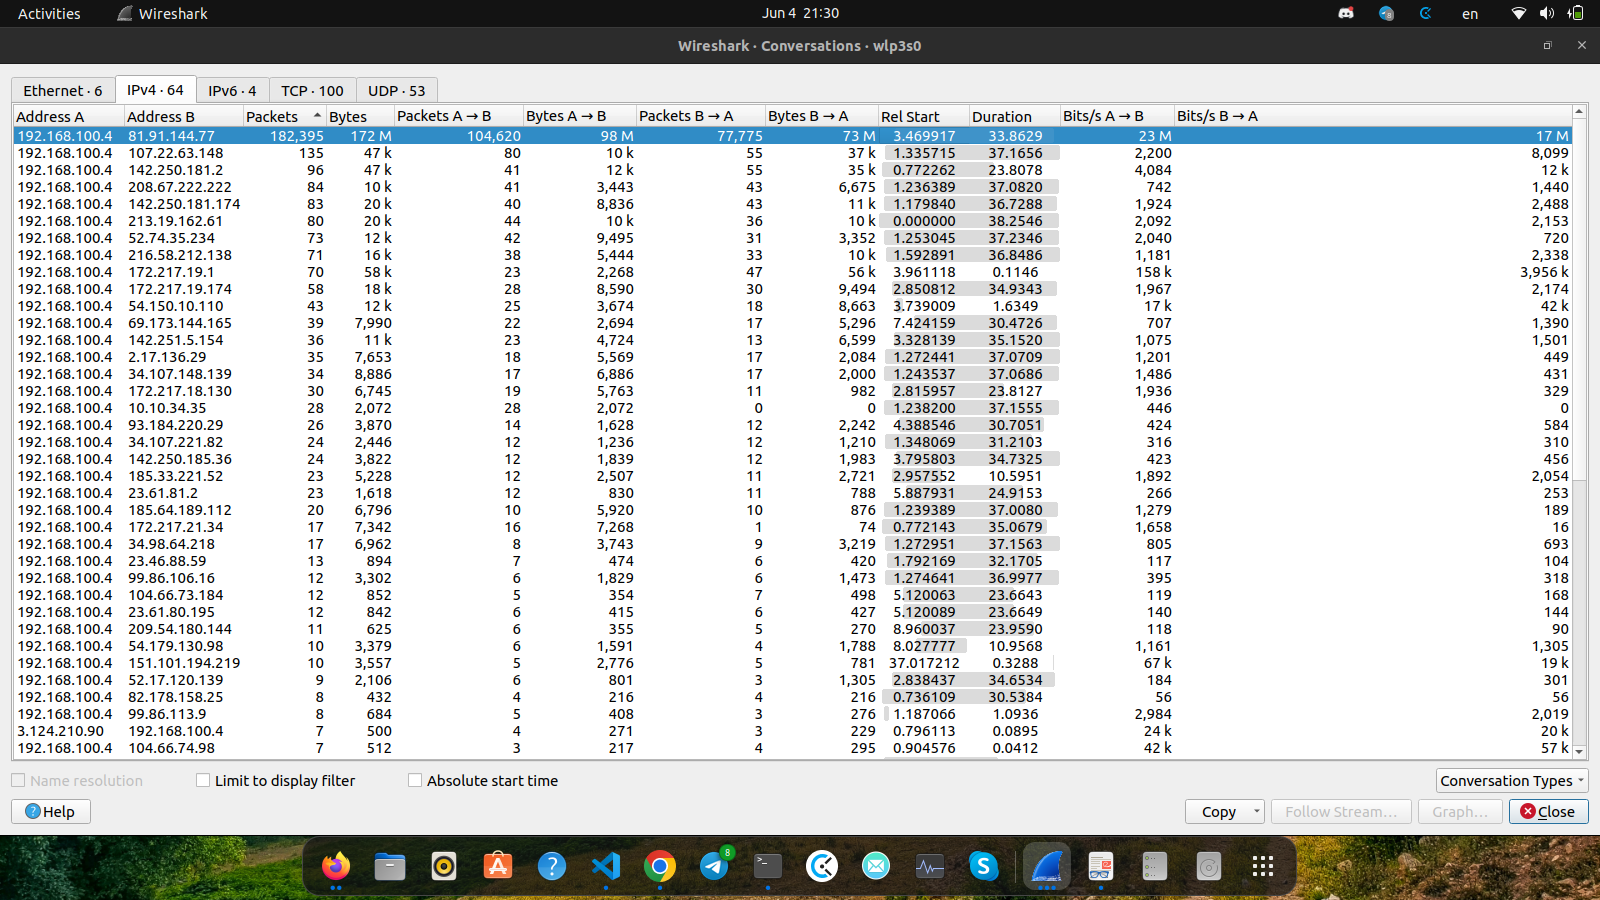
\includegraphics[width=\textwidth]{./resources/WSDelayTotal.png}
    \caption{Speed Test Total Time}
    \label{fig:WSDelayTotal}
\end{figure}

\section{}
RTMP or Real-Time Messaging Protocol is a protocol for streaming media over the Internet. It was primarily developed by Micromedia (which is now owned by Adobe Systems) and is used by Adobe Flash Media Server (FMS) to stream media to the client. It is TCP-base protocol and maintains persistent connections between the client and the server. Hence it has low delay and is reliable. It splits the media stream into multiple fragments and sends them to the client. The fragment size is dynamic and can be negotiated by the client and the server. RTMP also use several channels to separate the media stream. 

RTMP is used in transport-layer protocol like TCP and UDP.

The structure of RTMP packet is shown in the figure \ref{fig:RTMPPacket}. It contains the header and the body. The header itself is composed of basic header and chunk message header. The basic header contains composite byte, chunk type, and stream ID. The chunk message header contains metadata about the chunk such as message size, timestamp, and message type. The body contains the actual data.

\begin{figure}
    \centering
    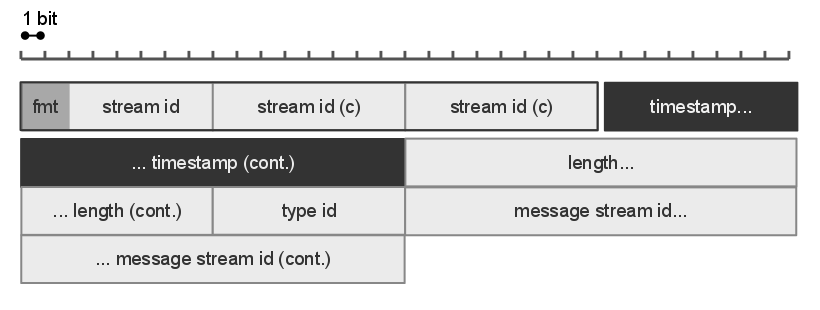
\includegraphics[width=0.5\textwidth]{./resources/RTMPPacket.png}
    \caption{RTMP Packet Structure}
    \label{fig:RTMPPacket}
\end{figure}

The handshake process is shown in the figure \ref{fig:RTMPHandshake}. It involves three packets. The first packet contains constant value 0x03 which represent the version of RTMP. Then the client without waiting for the response, sends the next packet which contains randomly generated value. Then both client and server echo the value back to each other. After that the handshake is completed.

\begin{figure}
    \centering
    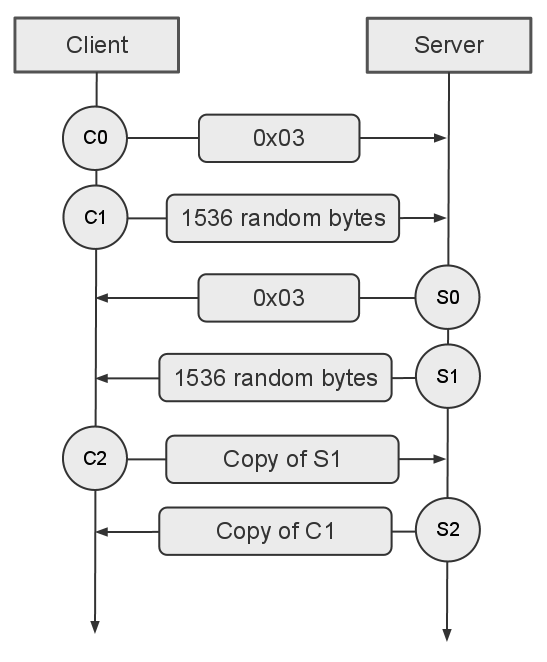
\includegraphics[width=0.5\textwidth]{./resources/RTMPHandshake.png}
    \caption{RTMP Handshake Diagram}
    \label{fig:RTMPHandshake}
\end{figure}

\end{document}